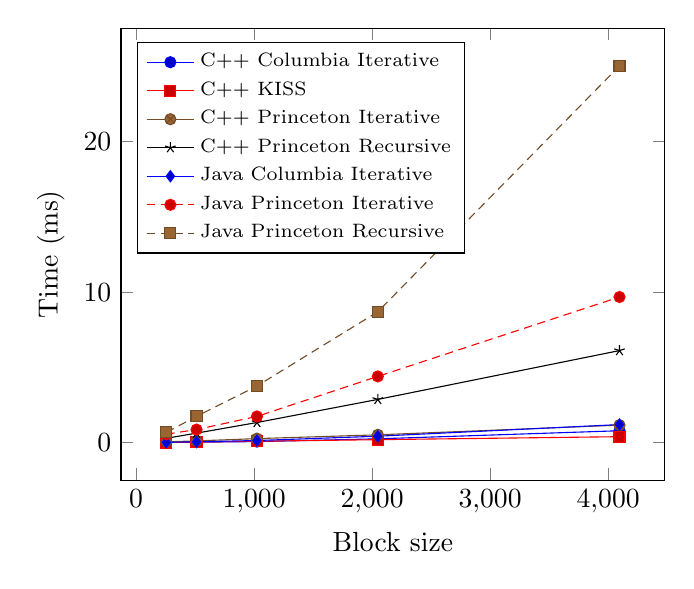
\begin{tikzpicture}
\begin{axis}[xlabel={Block size},ylabel={Time (ms)},width=0.70\linewidth,legend pos=north west,scaled y ticks = false,legend cell align=left,legend style={font=\scriptsize}]
\addplot coordinates {
(256, 0.0200)
(512, 0.0366)
(1024, 0.0773)
(2048, 0.2604)
(4096, 0.7974)
};
\addplot coordinates {
(256, 0.0182)
(512, 0.0461)
(1024, 0.0992)
(2048, 0.2047)
(4096, 0.4022)
};
\addplot coordinates {
(256, 0.0627)
(512, 0.1225)
(1024, 0.2744)
(2048, 0.5257)
(4096, 1.1701)
};
\addplot coordinates {
(256, 0.2978)
(512, 0.6379)
(1024, 1.3437)
(2048, 2.8773)
(4096, 6.1206)
};
\addplot coordinates {
(256, 0.0293)
(512, 0.0615)
(1024, 0.1484)
(2048, 0.4338)
(4096, 1.2071)
};
\addplot coordinates {
(256, 0.5698)
(512, 0.8758)
(1024, 1.7488)
(2048, 4.4055)
(4096, 9.6792)
};
\addplot coordinates {
(256, 0.6929)
(512, 1.7515)
(1024, 3.7688)
(2048, 8.6983)
(4096, 25.0276)
};
\legend{C++ Columbia Iterative,C++ KISS,C++ Princeton Iterative,C++ Princeton Recursive,Java Columbia Iterative,Java Princeton Iterative,Java Princeton Recursive}
\end{axis}
\end{tikzpicture}
